\documentclass[runningheads]{llncs}

% ---------------------------------------------------------------
% Include basic ECCV package
 
% TODO REVIEW: Insert your submission number below by replacing '*****'
% TODO FINAL: Comment out the following line for the camera-ready version
% \usepackage[review,year=2024,ID=3431]{eccv}
% TODO FINAL: Un-comment the following line for the camera-ready version
\usepackage{eccv}

% OPTIONAL: Un-comment the following line for a version which is easier to read
% on small portrait-orientation screens (e.g., mobile phones, or beside other windows)
%\usepackage[mobile]{eccv}


% ---------------------------------------------------------------
% Other packages

% Commonly used abbreviations (\eg, \ie, \etc, \cf, \etal, etc.)
\usepackage{eccvabbrv}

% Include other packages here, before hyperref.
\usepackage{graphicx}
\usepackage{booktabs}


\usepackage{graphicx}
\usepackage{multirow}
\usepackage{bbding}
\usepackage{balance}
\usepackage{diagbox}
\usepackage{soul}
\usepackage{colortbl}
\usepackage{circledsteps}
\usepackage{floatrow}
\usepackage{amsmath}
\floatsetup[table]{capposition=top}
% \usepackage{tabularx}
% \usepackage{caption}
% \usepackage[leftcaption]{sidecap}


% \usepackage{graphicx}
% \usepackage{subfigure}
\usepackage{amsmath}
\usepackage{amssymb}
% \usepackage{booktabs}
% \usepackage{bbm}
% % \usepackage[table]{xcolor}
% \usepackage[dvipsnames,svgnames,x11names,table]{xcolor} % colors
% % \usepackage[pagebackref,breaklinks,colorlinks]{hyperref}
% \newcommand{\xmark}{\ding{55}}%
% \usepackage{bbding}
% \newcommand{\rownumber}[1]{\textcolor{black}{#1}}
% \usepackage{wrapfig}
% \usepackage{multirow}
% \usepackage{transparent}
% \usepackage{tikz}



% The "axessiblity" package can be found at: https://ctan.org/pkg/axessibility?lang=en
\usepackage[accsupp]{axessibility}  % Improves PDF readability for those with disabilities.


% ---------------------------------------------------------------
% Hyperref package

% It is strongly recommended to use hyperref, especially for the review version.
% Please disable hyperref *only* if you encounter grave issues.
% hyperref with option pagebackref eases the reviewers' job, but should be disabled for the final version.
%
% If you comment hyperref and then uncomment it, you should delete
% main.aux before re-running LaTeX.
% (Or just hit 'q' on the first LaTeX run, let it finish, and you
%  should be clear).

% TODO FINAL: Comment out the following line for the camera-ready version
\usepackage[pagebackref,breaklinks,colorlinks,citecolor=eccvblue]{hyperref}
% TODO FINAL: Un-comment the following line for the camera-ready version
%\usepackage{hyperref}

% Support for ORCID icon
\usepackage{orcidlink}

\begin{document}

% ---------------------------------------------------------------
% TODO REVIEW: Replace with your title
%\title{UniMERNet: Enhancing Mathematical Expression Recognition in Real-World Scenarios} 
\title{UniMERNet: A Universal Network for Real-World Mathematical Expression Recognition}

% TODO REVIEW: If the paper title is too long for the running head, you can set
% an abbreviated paper title here. If not, comment out.
\titlerunning{UniMERNet: A Universal Network for Real-World MER}

% TODO FINAL: Replace with your author list. 
% Include the authors' OCRID for the camera-ready version, if at all possible.
% \author{First Author\inst{1}\orcidlink{0000-1111-2222-3333} \and
% Second Author\inst{2,3}\orcidlink{1111-2222-3333-4444} \and
% Third Author\inst{3}\orcidlink{2222--3333-4444-5555}}

\author{
    %Authors
    % All authors must be in the same font size and format.
   Bin Wang$^{*}$, 
   Zhuangcheng Gu$^{*}$, \\
   Chao Xu,
   Bo Zhang,
   Botian Shi,
   Conghui He$^{\dag}$
}

% TODO FINAL: Replace with an abbreviated list of authors.
\authorrunning{B. Wang \textit{et al.}}
% First names are abbreviated in the running head.
% If there are more than two authors, '\textit{et al.}' is used.

% TODO FINAL: Replace with your institution list.
% \institute{Princeton University, Princeton NJ 08544, USA \and
% Springer Heidelberg, Tiergartenstr.~17, 69121 Heidelberg, Germany
% \email{lncs@springer.com}\\
% \url{http://www.springer.com/gp/computer-science/lncs} \and
% ABC Institute, Rupert-Karls-University Heidelberg, Heidelberg, Germany\\
% \email{\{abc,lncs\}@uni-heidelberg.de}}

\institute{Shanghai AI Laboratory}

\maketitle

\newcommand\blfootnote[1]{
    \begingroup
    \renewcommand\thefootnote{}\footnote{#1}
    \addtocounter{footnote}{-1}
    \endgroup
}
\blfootnote{
\noindent $*$ Equal contribution. \\
$\dag$ Corresponding author: \href{heconghui@pjlab.}{\color{black}{heconghui@pjlab.org.cn}}
}

\begin{abstract}
This paper presents the UniMER dataset to provide the first study on Mathematical Expression Recognition (MER) towards complex real-world scenarios. The UniMER dataset consists of a large-scale training set UniMER-1M offering an unprecedented scale and diversity with one million training instances and a meticulously designed test set UniMER-Test that reflects a diverse range of formula distributions prevalent in real-world scenarios. Therefore, the UniMER dataset enables the training of a robust and high-accuracy MER model and comprehensive evaluation of model performance. Moreover, we introduce the Universal Mathematical Expression Recognition Network (UniMERNet), an innovative framework designed to enhance MER in practical scenarios. UniMERNet incorporates a Length-Aware Module to process formulas of varied lengths efficiently, thereby enabling the model to handle complex mathematical expressions with greater accuracy. In addition, UniMERNet employs our UniMER-1M data and image augmentation techniques to improve the model's robustness under different noise conditions. Our extensive experiments demonstrate that UniMERNet outperforms existing MER models, setting a new benchmark in various scenarios and ensuring superior recognition quality in real-world applications. The dataset and model are available at \url{https://github.com/opendatalab/UniMERNet}.

  
  \keywords{Mathematical Expression Recognition \and Length-Aware Module \and Data Augmentation}
\end{abstract}


\section{Introduction}
\label{sec:intro}

Mathematical Expression Recognition (MER), a key task in document analysis, aims to convert image-based mathematical expressions into corresponding markup languages such as LaTeX or Markdown. MER is important in applications such as scientific document extraction, where a robust MER model helps maintain document logical coherence. Unlike typical Optical Character Recognition (OCR) tasks, MER requires a more sophisticated understanding of complex structures, including superscripts, subscripts, and various special symbols.


Existing research has primarily focused on enhancing recognition accuracy for relatively simple rendered expressions~\cite{deng2017image} and handwritten data~\cite{mahdavi2019icdar,le2019pattern,wu2020handwritten,zhao2021handwritten} through a series of MER algorithms. 
Some researchers have begun to optimize MER algorithms by scaling up the training data and integrating them with transformer~\cite{vaswani2017attention} models, ensuring their applicability in diverse scenarios~\cite{kim2022ocr,pix2tex2022,blecher2023nougat,texify2023}. 
Other researchers have attempted to directly employ Large Vision-Language Models (LVLMs) for document content extraction, including MER~\cite{wei2023vary, blecher2023nougat}.
However, existing MER benchmarks~\cite{deng2017image,mahdavi2019icdar} primarily focus on simple printed expressions or handwritten image recognition.
Therefore, these models tend to struggle with diverse real-world expressions, such as lengthy equations and noisy scanned document screenshots. 



\begin{figure}[t]
  \centering
	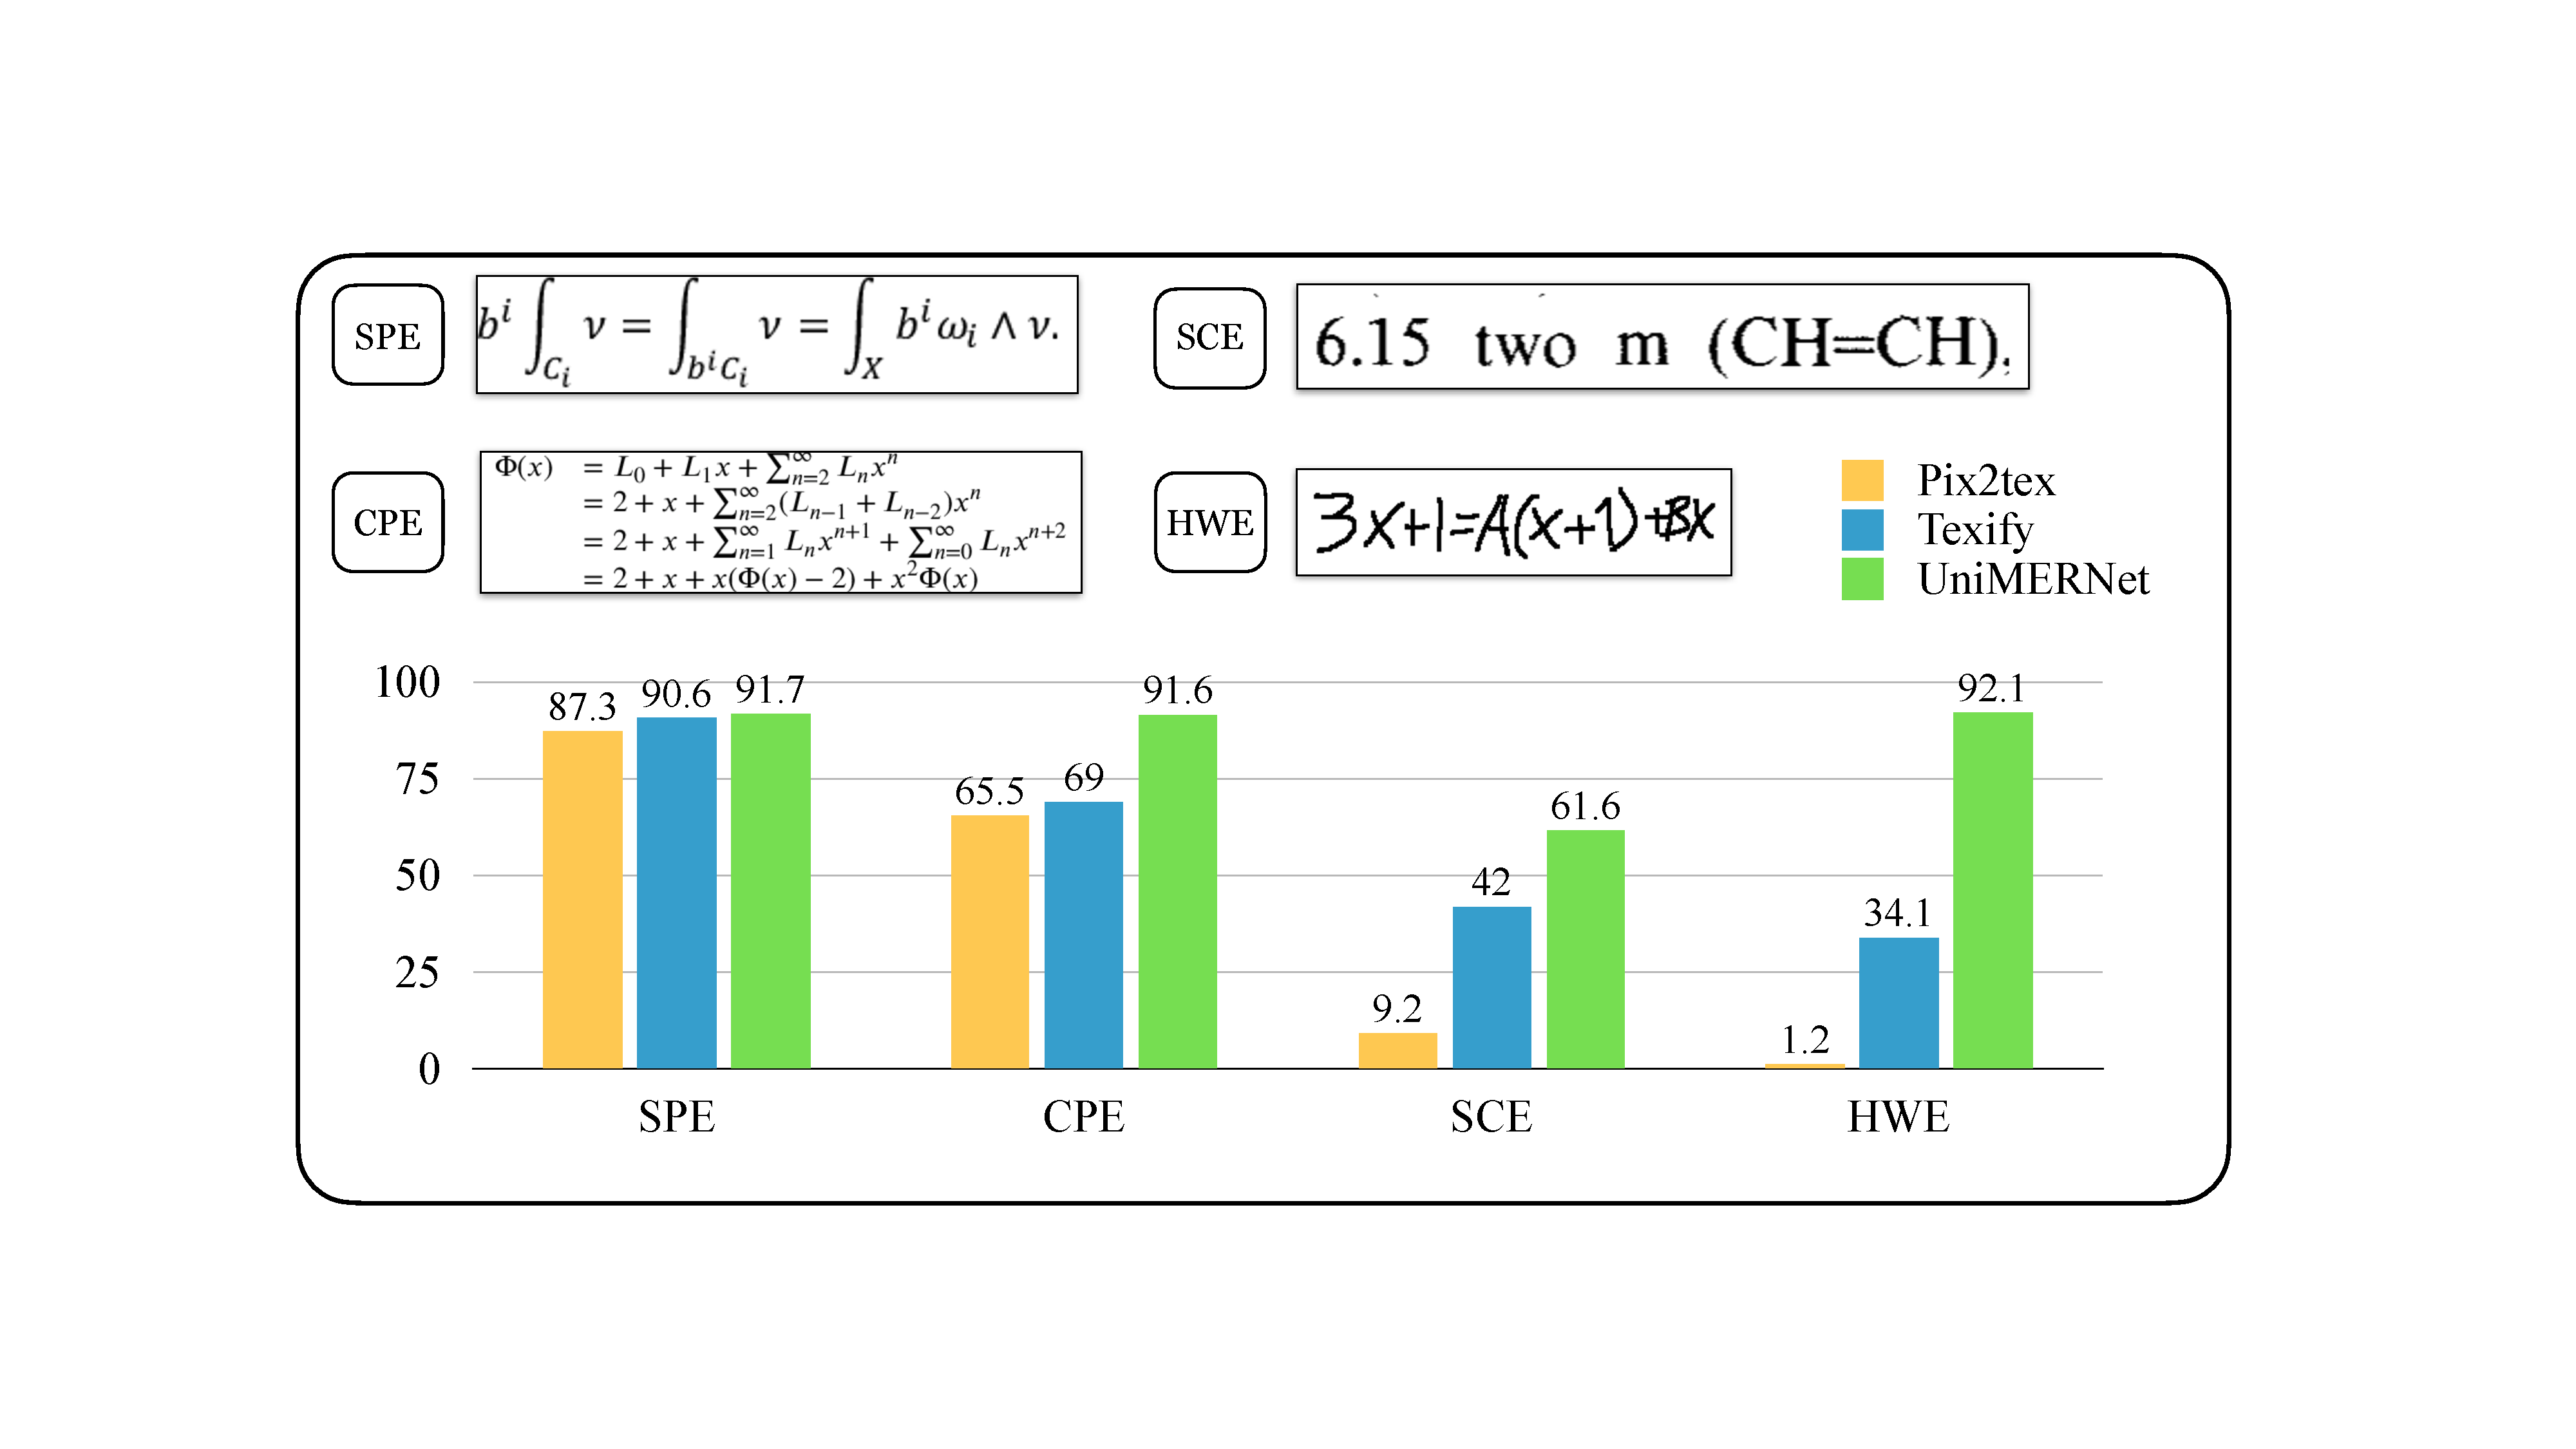
\includegraphics[width=0.95 \linewidth]{figures/fig1_bleu.pdf}
    \caption{Performance comparison (BLEU Score) of mainstream models and UniMERNet in recognizing real-world mathematical expressions: Evaluation across Simple Printed Expressions (SPE), Complex Printed Expressions (CPE), Screen-Captured Expressions (SCE), and Handwritten Expressions (HWE).}
  \label{fig:fig1_introduction}
  \vspace{-2pt}
\end{figure}

In practice, real-world scenarios require the handling of complex, long expressions and noisy, distorted images from scanned documents or webpage screenshots.
To fill this gap, we introduce a comprehensive benchmark, UniMER-Test, which extends the existing test set with longer and real-world scenario expressions. 
Our benchmark stimulates the progress of MER in robustness and practical usage.
As depicted in ~\cref{fig:fig1_introduction}, we conducted an exhaustive evaluation of state-of-the-art MER methods~\cite{pix2tex2022,texify2023} using our novel benchmark, UniMER-Test. 
These methods demonstrate remarkable competence in recognizing simple printed expressions.
However, their performance noticeably declines when tested with more complex printed expressions, particularly long formulas. 
The performance degradation becomes even more pronounced when these methods are applied to real-world expressions, such as screen-captured expressions embedded in noisy backgrounds and handwritten expressions. 
Moreover, large vision-language models such as Nougat~\cite{blecher2023nougat} and Vary~\cite{wei2023vary}, despite their capacity for convenient end-to-end document content extraction, exhibit only mediocre performance in MER.

% Version 3
To address these challenges, we first introduce the UniMER dataset, an extensive collection tailored for Mathematical Expression Recognition (MER), featuring 1 million meticulously curated expressions. Designed to both complement and validate the advancements in MER, this dataset includes the comprehensive UniMER-1M training samples and the thorough UniMER-Test sets, aiming to stimulate further research by offering a broader diversity of expressions compared to existing datasets.
Together with the dataset, we propose UniMERNet, a model attuned to the sequence lengths of expressions with its additional length-aware module (LAM). UniMERNet leverages context information regarding the length of an expression prior to prediction, allowing it to generate an expression with sequence length matching the visual feature of the input images. This model is further enhanced through image augmentation techniques, significantly boosting its performance in real-world applications. The main contributions of this paper are as follows:
\begin{itemize}
\item We introduce \textbf{UniMER}, a universal MER dataset, with the training set UniMER-1M and the test set UniMER-Test, which encompasses all types of expressions in practical situations, offering a diverse and comprehensive foundation for MER model development and evaluation.
\item We present \textbf{UniMERNet}, a novel MER framework based on the encoder-decoder structure, with an innovative sequence Length-Aware Module to improve the model's ability to handle a wider range of expressions than existing models
\item Validation of UniMERNet's superior performance through extensive experiments, establishing it as the new benchmark in open-source MER solutions by outperforming existing models in a variety of scenarios.

\end{itemize}



\section{Related Work}
\subsection{Machine Learning-Based Methods}

Several decades ago, researchers began recognizing the uniqueness and significance of Mathematical Expression Recognition (MER), leading to the initiation of corresponding studies. Anderson~\cite{anderson1967syntax} pioneers an approach to MER in irregular documents, introducing a parsing algorithm for two-dimensional character configurations. Miller \& Viola ~\cite{Miller_Viola_1998} propose an efficient system that integrates specialized character segmentation with the intrinsic grammar of the mathematical layout language. Chan \textit{et al.}~\cite{Chan_Yeung_1999} develop an online MER system, incorporating an error detection and correction mechanism to handle lexical, syntactic, and semantic errors. INFTY~\cite{suzuki2003infty} is an integrated OCR system for mathematical documents that achieves high accuracy in character recognition through a series of novel techniques. Despite the innovative works during this stage, the precision of MER remains limited due to the limitations of handcrafted features in traditional machine learning.


\subsection{CNN-Based Deep Learning Methods}

% \subsection{Early Deep Learning-Based Methods}
With the advent and development of deep learning, a series of MER algorithms based on Convolutional Neural Networks (CNN)~\cite{krizhevsky2012imagenet,simonyan2015very} are proposed. Deng \textit{et al.}~\cite{deng2017image} introduce an encoder-decoder model for OCR, leveraging a scalable coarse-to-fine attention mechanism. They present a new dataset, IM2LATEX-100K, demonstrating the superiority of their approach over traditional OCR systems in handling non-standard tasks. The WAP~\cite{zhang2017watch} model learns mathematical expression grammar and handles symbol segmentation autonomously, with its learned alignments closely mirroring human intuition. The PAL-v2~\cite{wu2020handwritten} model employs paired adversarial learning to recognize handwritten mathematical expressions, effectively manage style variations, and show solid performance on the CROHME dataset. Zhang \textit{et al.}~\cite{zhang2020tree} propose a tree-structured decoder for image-to-markup tasks, exhibiting superior performance over traditional string decoders in handling complex tree-structured markups, while maintaining flexibility for various sequence-to-sequence problems. Leveraging bi-directional learning, Zhao \textit{et al.}~\cite{zhao2021handwritten} and Bian \textit{et al.}~\cite{bian2022handwritten} effectively enhance the recognition performance of their encoder-decoder models for MER, thereby promoting advancements in the field of Handwritten Mathematical Expression Recognition (HMER). The CAN~\cite{li2022counting} enhances HMER by integrating a weakly-supervised counting module into the encoder-decoder model, optimizing HMER and symbol counting concurrently for improved performance. By employing data augmentation strategies, including distortion, decomposition, and scale augmentation techniques, Le \textit{et al.}~\cite{le2019pattern} and Li \textit{et al.}~\cite{li2020improving} substantially enhance the performance of MER, effectively addressing the issue of data scarcity. Deep learning-based algorithms significantly improve precision compared to traditional machine learning methods. However, current MER focuses more on handwritten formulas, overlooking those in documents and screenshots.

\subsection{Transformer-Based Deep Learning Methods}

% \subsection{Modern Deep Learning-Based Methods}
In recent years, with the rapid development of Transformer~\cite{vaswani2017attention} and large vision-language models~\cite{zhu2023minigpt,liu2024visual,dong2024internlm,liu2023improved}, researchers have gradually realized that a wealth of knowledge information exists in document data, which is crucial for further enhancing the performance of large models. Therefore, some researchers have begun to study how to extract document information. Donut~\cite{kim2022ocr} proposes an end-to-end document information extraction model that can directly convert input document images into structured outputs without relying on OCR. Nougat~\cite{blecher2023nougat} employs more rule-based auto-generated image-to-markup samples to train an end-to-end transformer-based encoder-decoder model. This model is specifically designed to transcode document pages into markup language. Vary~\cite{wei2023vary} is a fine-grained perception-capable multimodal large model that can be used for document content parsing. However, these methods have not considered the special nature of mathematical expressions compared to general text, and their MER capabilities are relatively weak. Therefore, Pix2tex~\cite{pix2tex2022} and Texify~\cite{texify2023}, based on a large number of rendered mathematical expressions, train encoder-decoder models, which work well on rendered mathematical expressions in documents. However, these methods often fail for complex mathematical expressions, and their recognition results are significantly reduced for noisy mathematical expressions under screenshots. The MER model proposed in this paper takes into account various situations, aiming to build a robust and practical MER model.


 \begin{table*}[t]
    \renewcommand\arraystretch{0.5}
    \centering
    \caption{Statistical comparison of the MER dataset. ``Max Length'' and ``Avg Length'' mean the maximum length and average string length of the mathematical expression.}
    \label{tab:tab1_statistic}
    \begin{tabular}{l|c|c|c|c|c}%l=left, r=right,c=center分别代表左对齐,右对齐和居中,字母的个数代表列数
    \toprule[1.0pt] 
    \textbf{Dataset}   & \textbf{ Type }& \textbf{ Train Size }&  \textbf{ Test Size } & \textbf{ Max Len } & \textbf{ Avg Len }  \\ \midrule[1pt]
    HME100K  & \multirow{2}{*}{HWE}         & 74,502    & 24,607    & 311  & 24.05  \\
    CROHME         &                        & 8,836     & 3233      & 147  & 22.27  \\  \midrule[0.5pt]
    IM2LATEX-100K  & \multirow{2}{*}{SPE}   & 83,883    & 10,354    & 440  & 96.01  \\  
    Pix2tex        &                        & 158,480   & 30,637    & 2949 & 93.35 \\  \midrule[0.5pt]
    UniMER-1M     & Mixed                  & 1,061,791 & 23,757    & 7037 & 79.48  \\
    \bottomrule[1.0pt]
    \end{tabular}
    \vspace{-5pt}
\end{table*}


\section{UniMER Dataset}

The UniMER dataset is tailored to tackle the challenge of formula recognition diversity in real-world scenarios.
The dataset is divided into two subsets: the UniMER-1M training set and the UniMER-Test testing set.
The UniMER-1M training set covers a wide array of mathematical expressions encountered in real-world situations.
Meanwhile, UniMER-Test facilitates comprehensive, accurate, multi-dimensional evaluation. 


Specifically, UniMER-1M comprises 1,061,791 Latex-Image sample pairs, encompassing both short and complex, long formula expressions. 
A crucial aspect of its construction was the careful balance of different length distributions.
This equilibrium is instrumental in enabling models trained on UniMER-1M to improve their overall recognition accuracy and generalization capabilities significantly.
UniMER-Test is constructed exclusively for the comprehensive evaluation of MER in real-world scenarios. It offers a detailed evaluation of MER from four dimensions, encompassing 6762 Simple Printed Expressions (SPE), 5,921 Complex Printed Expressions (CPE), 4,774 Screen Capture Expressions (SCE), and 6,332 Handwritten Expressions (HWE). This diverse range of expressions, totaling 23,789 samples, ensures a thorough evaluation of MER's performance.


As shown in \cref{tab:tab1_statistic}, the UniMER dataset presents two notable enhancements over existing datasets. Firstly, the UniMER-1M training set is distinguished by its inclusion of formulas of varied lengths and complex expressions, which are scarcely represented in current datasets, encompassing a total of 1 million instances - a significant increase from the previously largest open-source dataset's 158,480 formulas. Secondly, the UniMER-Test evaluation set encompasses samples from various dimensions, offering a more realistic and comprehensive assessment of model performance in practical applications.


The UniMER-1M dataset includes the following types of formulas:

\begin{itemize}
    \item SPE. These are formula images rendered from simple LaTeX expressions. They are characterized by uniform font size, clean background, and relatively short formulas, as shown in the first row of \cref{fig:fig2_example}.   
    
    \item CPE. These are formula images rendered from complex, long LaTeX expressions. They are characterized by uniform font size, clean background, and complex, longer formulas, as shown in the second row of \cref{fig:fig2_example}.
    
    \item SCE. These are screen-captured images of formulas from documents and the web. They are characterized by inconsistent fonts and sizes, background noise, and image deformation, as seen in the third row of  \cref{fig:fig2_example}.
    
    \item HWE. These are collected from referenced handwriting recognition datasets~\cite{mouchere2014icfhr,mouchere2016icfhr2016,mahdavi2019icdar,yuan2022syntax}. They are complex and diverse, with varying backgrounds, but are relatively short, as shown in the fourth row of  \cref{fig:fig2_example}.

\end{itemize}


\subsection{Data Collection Process}

\subsubsection{Printed Rendered Expressions (SPE, CPE)}


The assembly of our dataset began with the public dataset provided by Pix2tex~\cite{pix2tex2022}, which served as the basis for our SPE. Recognizing the limitations of the Pix2tex dataset in terms of volume and complexity, we embarked on a data augmentation process. For the SPE, we expanded the base data by sourcing additional LaTeX expression source codes from platforms such as Arxiv~\footnote{https://arxiv.org/}, Wikipedia~\footnote{https://www.wikipedia.org/}, and Physics/Math StackExchange~\footnote{https://stackexchange.com}. These codes underwent a regularization process \cite{deng2017image} to resolve any LaTeX syntax ambiguities before being compiled into expression PDF files in various fonts using XeLaTeX~\footnote{https://www.ctan.org/pkg/xetex}. Uncompilable expressions were discarded. Subsequently, ImageMagic's conversion function~\footnote{https://imagemagick.org/} was utilized to transform these images into expressions with multiple DPIs, with data balancing ensuring an even distribution of different lengths.

Following this data expansion pipeline, we sampled 725,246 simple formulas from the augmented data and combined them with the Pix2tex training set to form the SPE training data. The Pix2tex test set is designated as the SPE test data. In contrast, the CPE is derived independently of the Pix2tex dataset. We randomly selected 110,332 complex formulas from the expanded data to create the UniMER-1M-CPE and UniMER-Test-CPE.


\begin{figure}[t]
  \centering
	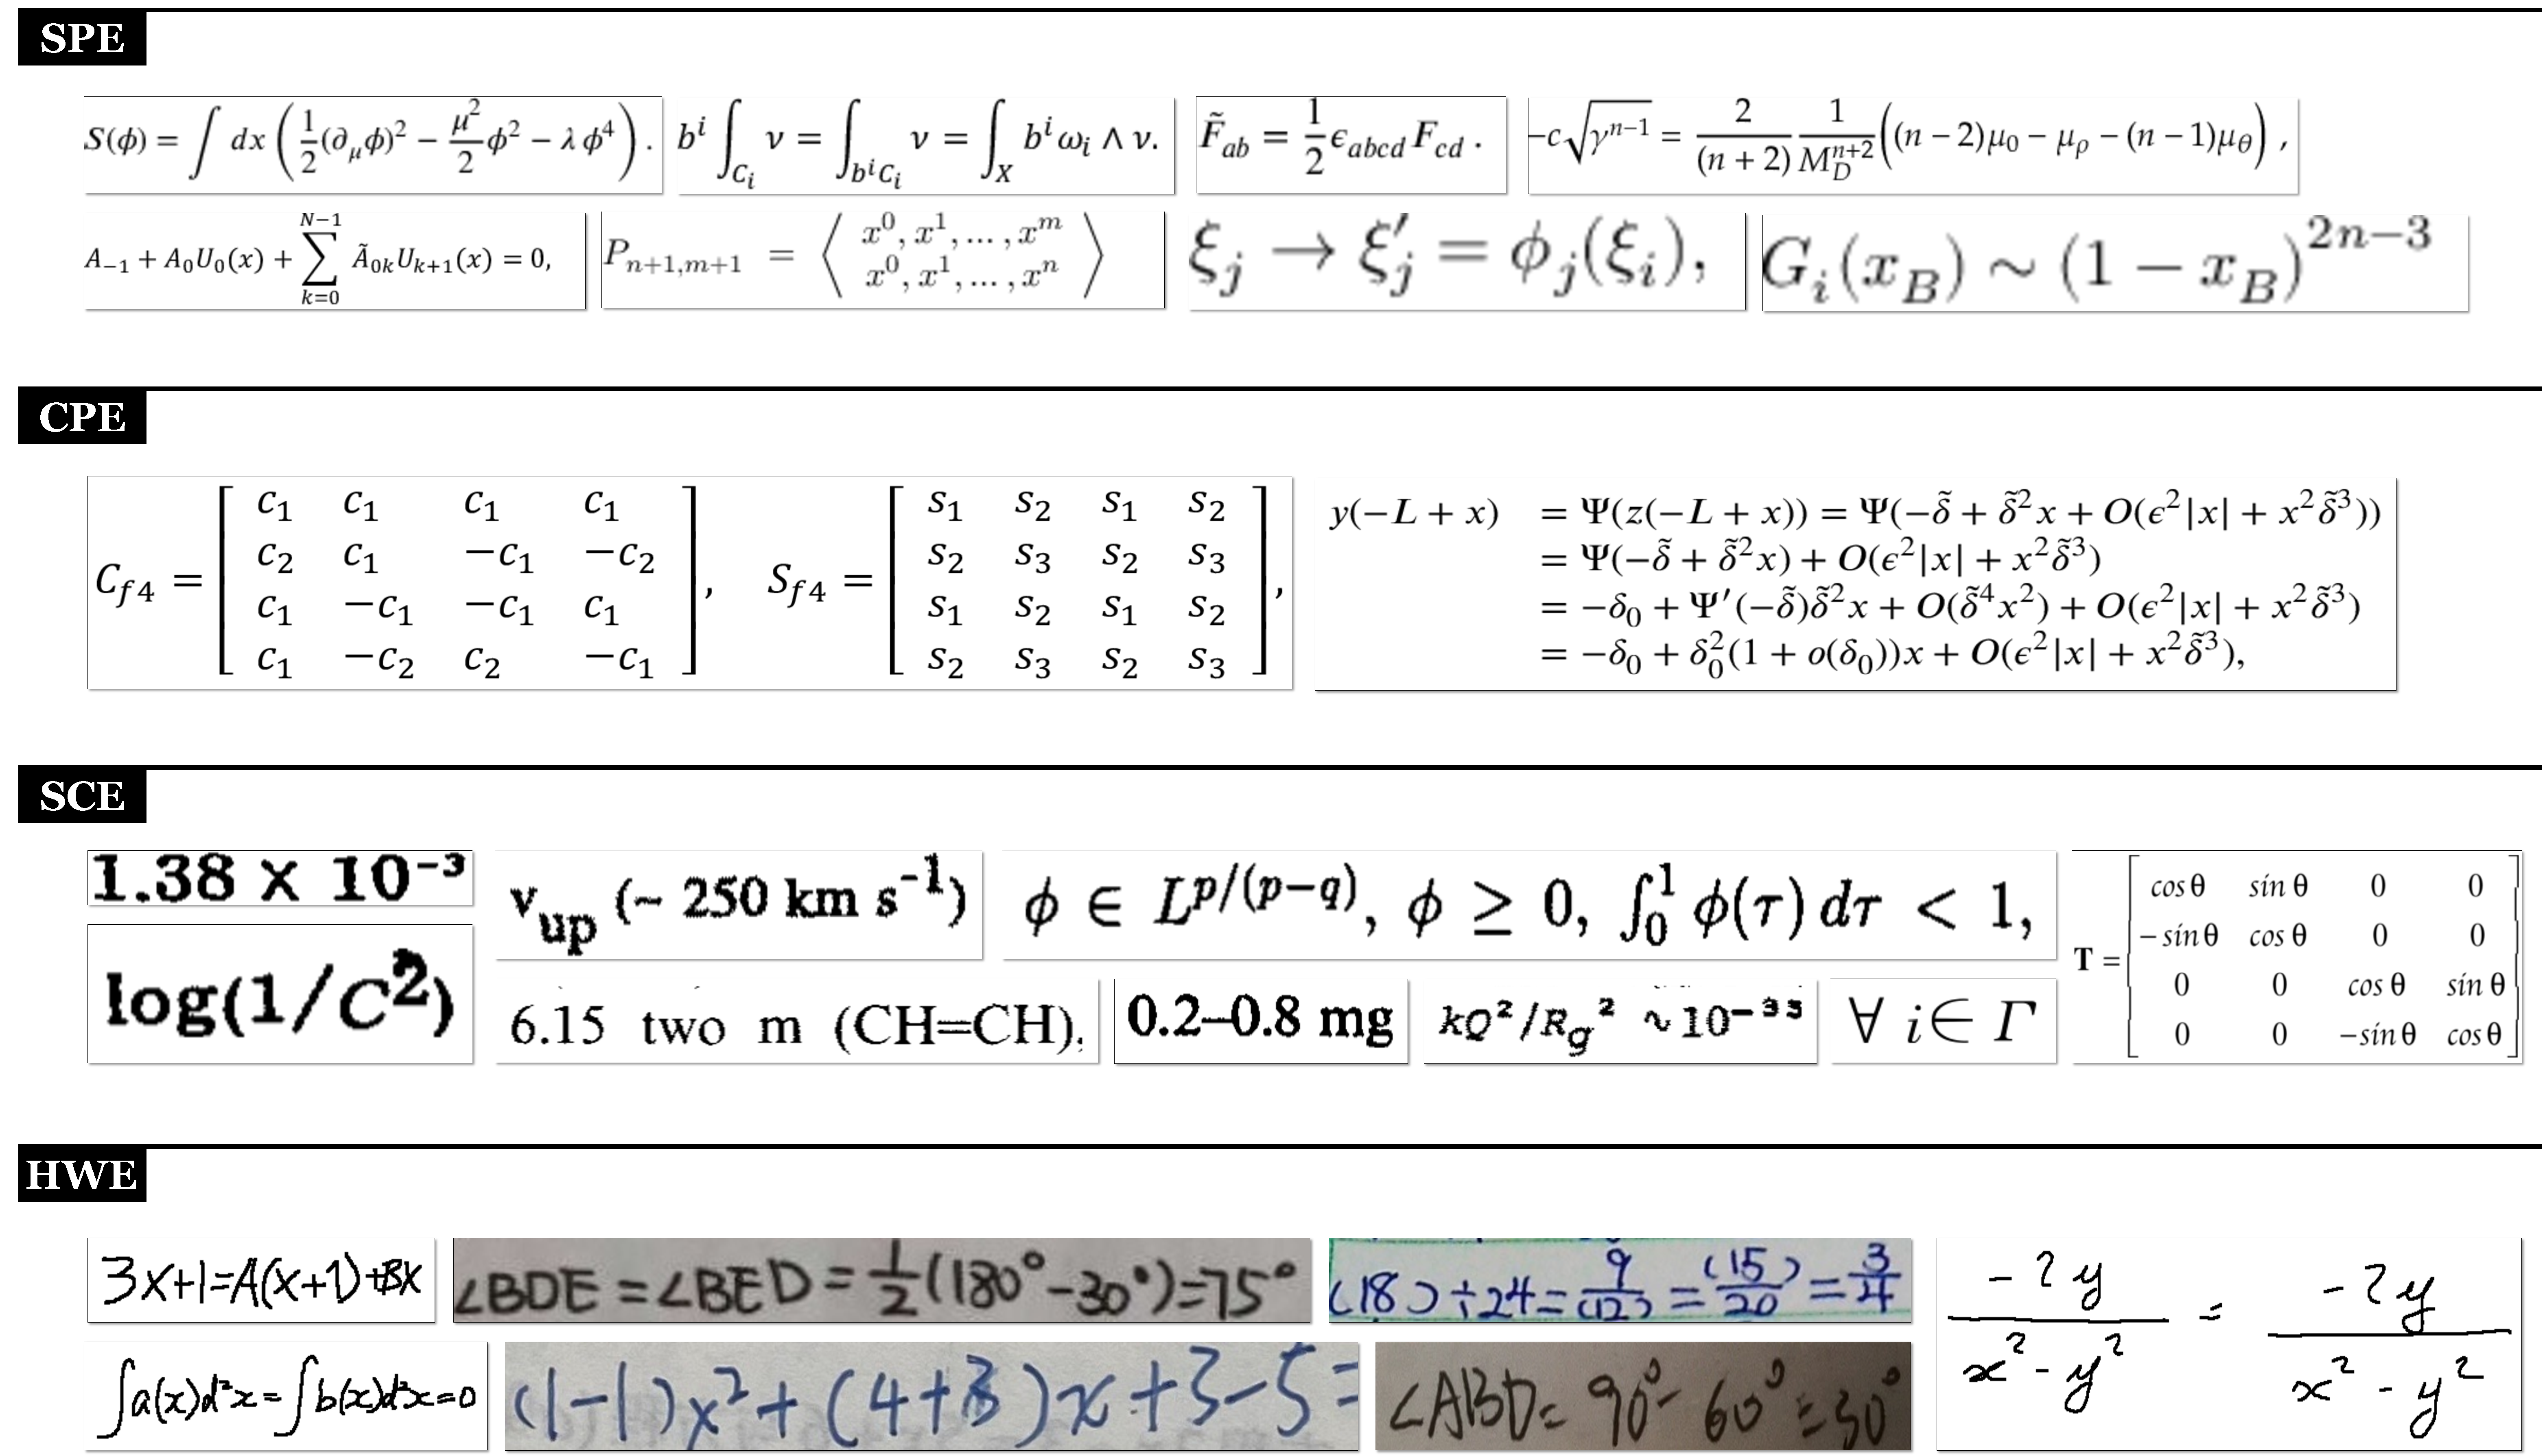
\includegraphics[width=0.95 \linewidth]{figures/fig2_unimernet_data.pdf}
    \caption{UniMER-1M: A comprehensive dataset for MER with Simple Printed Expressions (SPE), Complex Printed Expressions (CPE), Screen Capture Expressions (SCE), and Handwritten Expressions (HWE).}
  \label{fig:fig2_example}
\end{figure}




\subsubsection{Screen-Captured Expressions (SCE)}

For SCE, we compiled a diverse collection of 1,000 PDF pages, encompassing a spectrum of content types in both Chinese and English, such as books, papers, textbooks, magazines, and newspapers. This diverse collection ensured a broad range of fonts, sizes, and backgrounds for the formulas. We employed two annotators to identify and label the formula boxes in the documents, and automatically capture the content within. This resulted in over 6,000 formula boxes, which were then processed through Mathpix~\footnote{https://mathpix.com/} for formula recognition. Manual corrections were applied based on recognition results, and the LaTeX annotations were cross-verified by two annotators. Redundant formulas were identified and removed, yielding 4,744 unique SCEs to be used as the SCE test set.


\subsubsection{Handwritten Expressions (HWE)}

For HWE, we leveraged the existing public datasets CROHME~\cite{mouchere2014icfhr,mouchere2016icfhr2016,mahdavi2019icdar} and HME100K~\cite{yuan2022syntax}. CROHME, a widely recognized dataset in the HMER field, originated from the handwritten digit recognition competition and includes 8,836 training expressions and 3,332 test expressions. HME100K, a real-world handwritten expression dataset, comprises 74,502 training and 24,607 test images. Given the high accuracy of these datasets' annotations, we combined them to form our HWE data. Specifically, the HWE training set incorporated 8,836 training formulas from CROHME and 74,502 training formulas from HME100K, totaling 83,338 training samples. The HWE test set comprised 3,332 test set formulas from CROHME and a 3,000 formula samples from the HME100K test set, resulting in a total of 6,332 test formulas.


\begin{figure}[tb]
  \centering
	
\includegraphics[width=0.95 \linewidth]{figures/fig3_distribution.png}
    \caption{Formula string length distribution across different datasets.}
  \label{fig:fig4_distrib}
  \vspace{-3pt}
\end{figure}
\vspace{-10pt}

% TODO: 这一部分移到合成数据的地方
\subsection{Diversified Training Data Sampling} 


Existing formula datasets, such as HWE (CHROME \& HME100K)~\cite{mouchere2014icfhr,mouchere2016icfhr2016,mahdavi2019icdar}, IM2LATEX~\cite{deng2017image}, and Pix2tex~\cite{pix2tex2022} predominantly comprise rendered and handwritten formulas. 
However, these datasets exhibit limitations in terms of formula length and complexity. For instance, Pix2tex mainly contains regular formulas and lacks extremely short or complex long formulas. 
On the other hand, handwritten formulas are typically short while diverse in handwriting styles, with none exceeding 256 characters.
To overcome these limitations, we have enriched our UniMER-1M dataset with a comprehensive range of additional formulas. These formulas have been carefully sampled from diverse sources such as Arxiv and Wikipedia, ensuring a balanced distribution of formula lengths of varying complexity. 
The length-aware sampling strategy equips the model trained on UniMER-1M to recognize formulas across a broad complexity spectrum, thereby enhancing its applicability.  The distribution of IM2LATEX, Pix2tex, HWE, and our UniMER-1M datasets can be seen in ~\cref{fig:fig4_distrib}.


\section{Methods}

Mathematical expressions, originating from various sources such as electronic documents, scanned images, screenshots, and photographs, are presented against diverse backgrounds and image representations. These expressions can range from single symbols to highly complex, lengthy formulas. Although many existing algorithms are optimized for specific types of formulas, our study aims to address a broad spectrum of formula recognition problems that arise in real-world scenarios. To this end, we propose \textbf{UniMERNet}, a novel architecture capable of processing formulas of all types effectively. UniMERNet, as illustrated in \cref{fig3:archtecture}, adopts the transformer-based encoder-decoder architecture~\cite{kim2022ocr} as its foundational framework.


\begin{figure}[tb]
  \centering
  %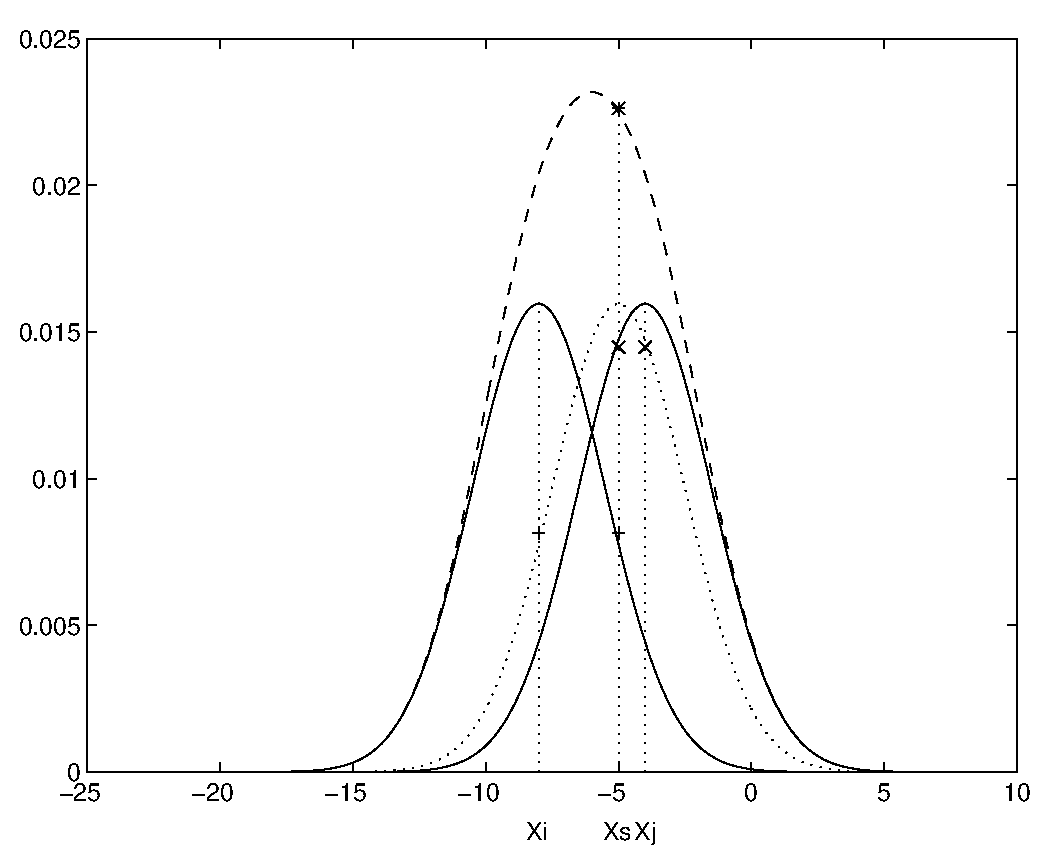
\includegraphics[height=6.5cm]{eijkel2}
	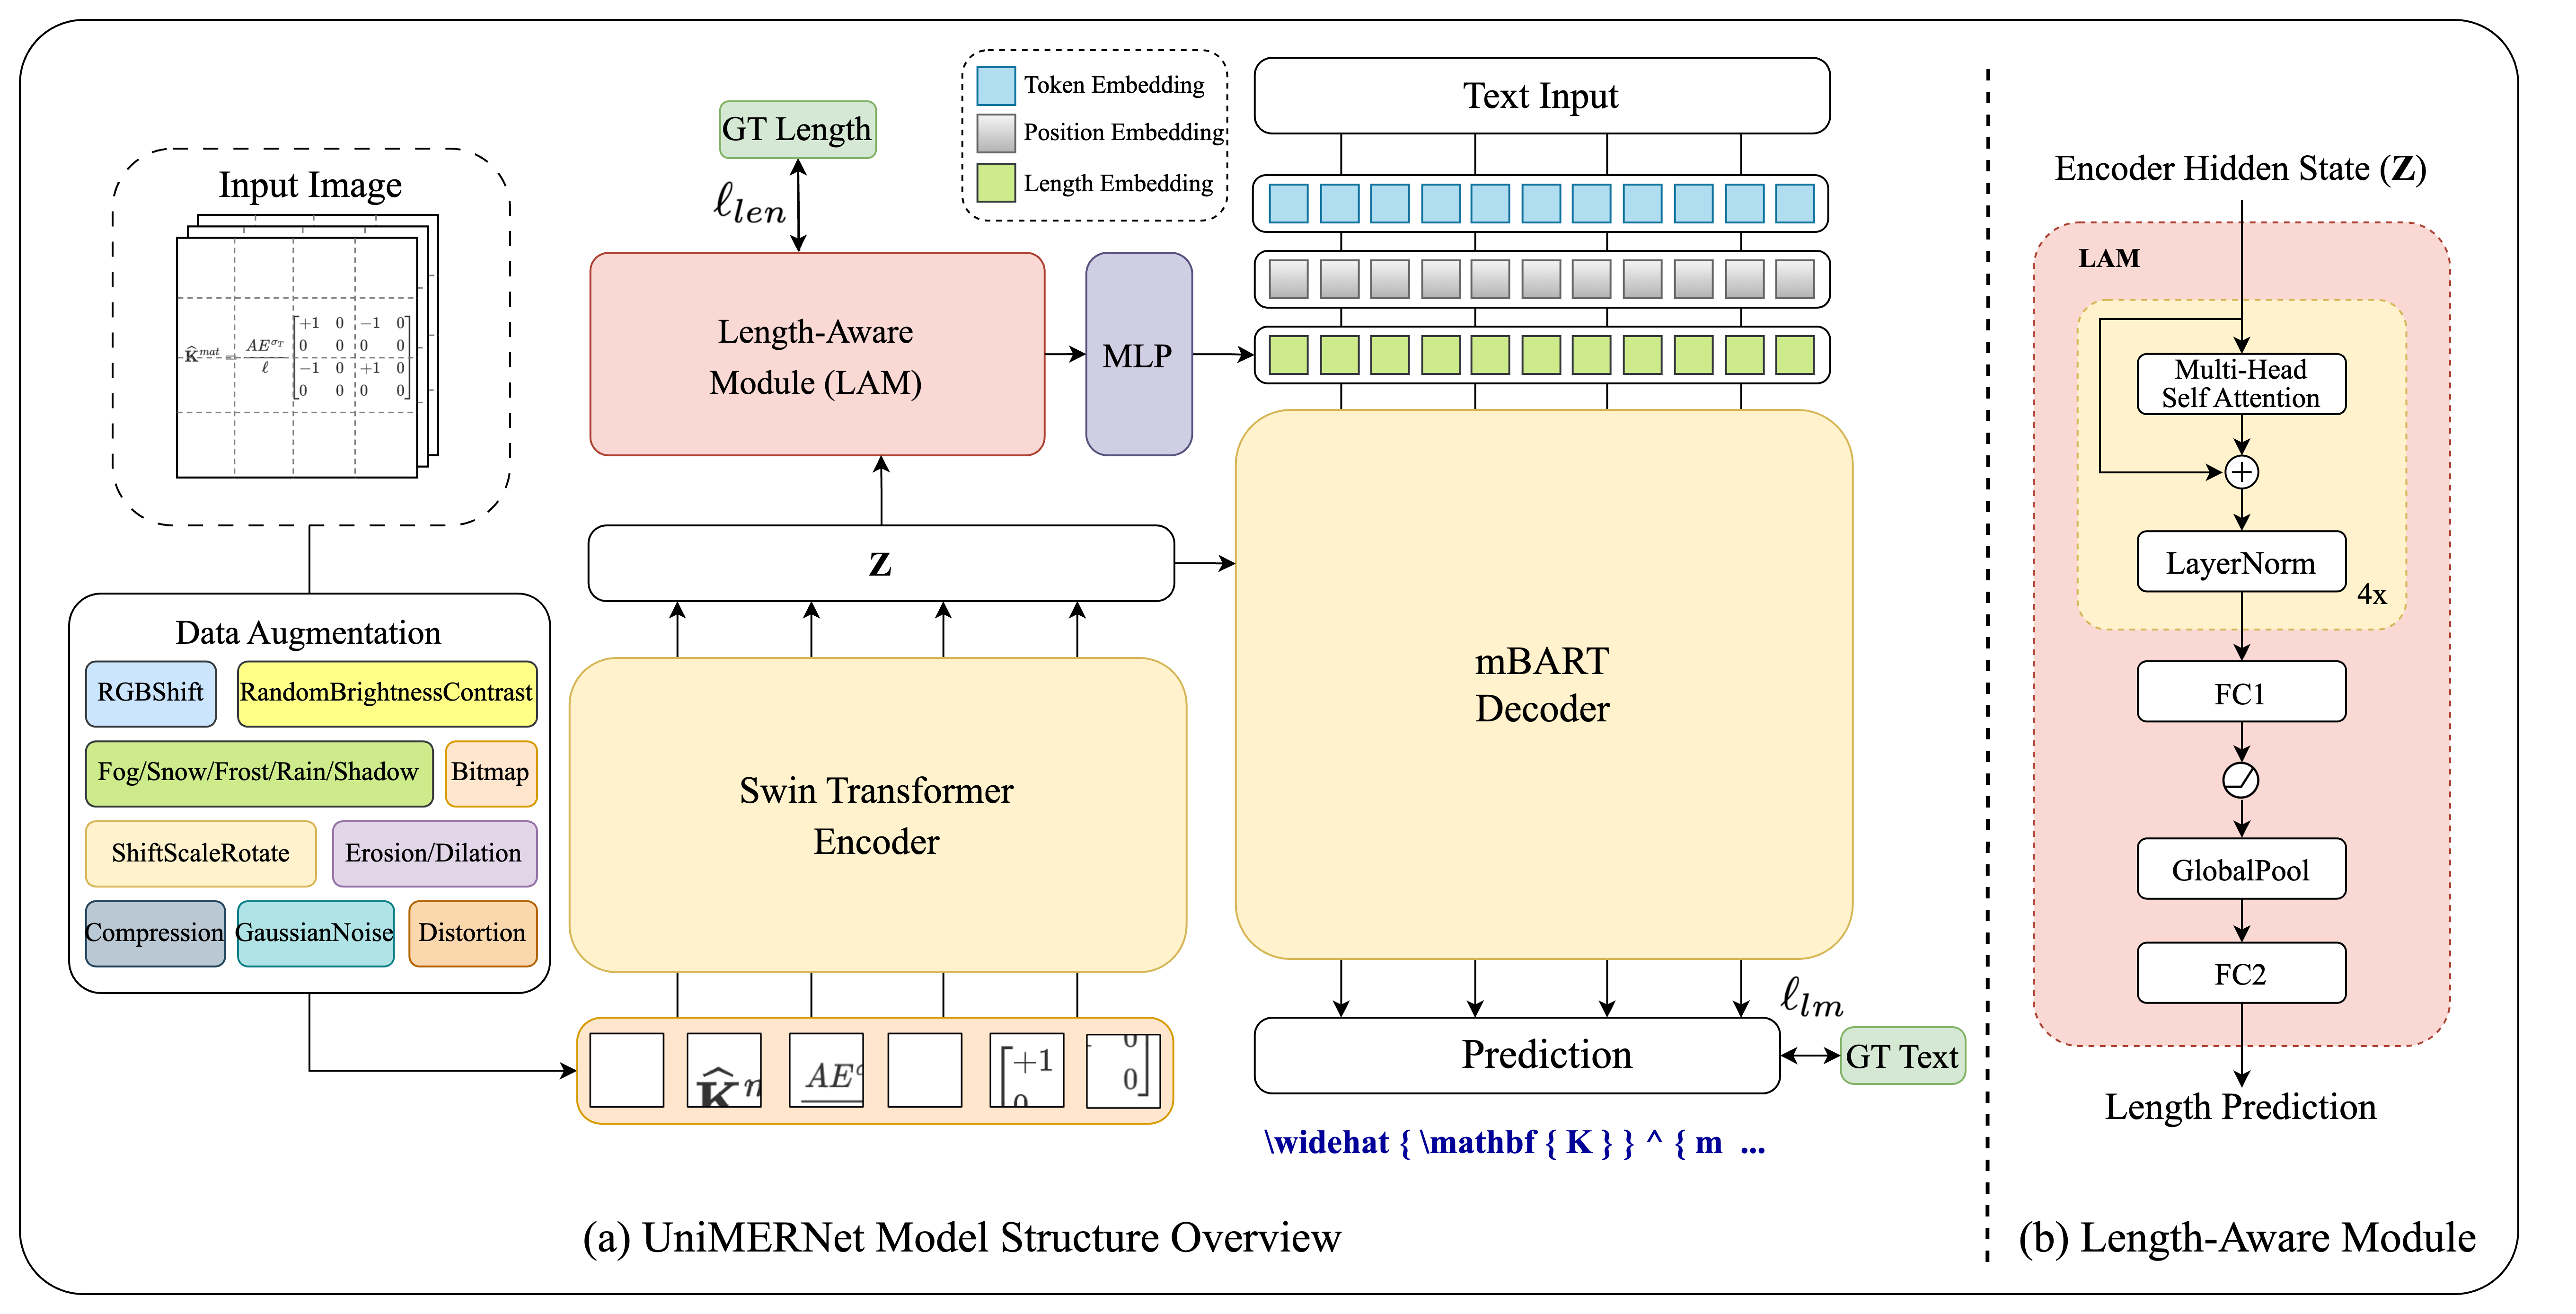
\includegraphics[width=0.98 \linewidth]{figures/fig4_UniMERNet.png}
    \caption{UniMERNet architecture and detailed view of Length-Aware Module.}
  \label{fig3:archtecture}
  \vspace{-4pt}
\end{figure}

During the training phase, each input formula image $\mathbf{I} \in \mathbb{R}^{3 \times H_0 \times W_0}$ undergoes an image augmentation module, which transforms a singular image representation into a diverse set of images, effectively addressing varied representations of formulas in real-world scenarios. The Swin Transformer~\cite{liu2021swin} encoder then processes the image to generate the feature vector $\mathbf{Z}$, which is fed into two distinct modules. The mBART~\cite{lewis2019bart} decoder receives the feature vector $\mathbf{Z}$ and interacts with the output text sequence via a cross-attention mechanism, facilitating the generation of the predicted formula. Simultaneously, the Length-Aware Module utilizes the feature vector to estimate the sequence length corresponding to the original formula image. This length information is encoded and incorporated into the decoder's input, providing additional context guiding the decoder in generating the formula. The decoder combines the feature vector $\mathbf{Z}$, token embedding, position embedding, and length embedding to predict the formula. The loss function includes both the text sequence matching loss and the formula length prediction loss, defined as:
\begin{equation}
    \mathcal{L} = \lambda_1 \ell_{lm} + \lambda_2 \ell_{len},
\end{equation}
where the $\ell_{lm}$ and $\ell_{len}$ correspond to language modeling loss and length loss respectively. For language modeling loss, we adopt a cross-entropy loss which minimise discrepancy between the predicted probability distribution of the next token and the actual distribution observed in the training data. Meanwhile, the length loss, $\ell_{len}$, use SmoothL1 Loss to regularize the predicted length of the mathematical expressions, ensuring that the model generates length prediction matching with the visual features from encoder. The definition of two losses are given by:
\begin{equation}
    \ell_{lm}(\hat{y}, y) = -\sum_{c=1}^{C} y_{o,c} \log(\hat{y}_{o,c}),
\end{equation}
\begin{equation}
    \ell_{len}(\hat{y}, y) = 
    \begin{cases} 
        0.5(\hat{y} - y)^2, & \text{if } |\hat{y} - y| < 1 \\
        |\hat{y} - y| - 0.5, & \text{otherwise}.
    \end{cases}
\end{equation}



Our UniMERNet, anchored by the encoder-decoder Transformer architecture, provides a robust solution to the challenges of formula recognition in diverse real-world scenarios. It incorporates an innovative Length Awareness Module (LAM) that estimates the formula length from the feature vector, enhancing the mBART decoder's ability to generate accurate predictions across a wide range of formula lengths. Complemented by our data expansion and image augmentation, UniMERNet effectively addresses the varied representations of formulas, demonstrating remarkable robustness and versatility. 
The following sections delve into the LAM and data augmentation techniques, underscoring their roles in enhancing UniMERNet's performance.

\subsection{Length Awareness Module}

Predicting real-world mathematical expressions, which range from simple symbols to complex sequences, is challenging in real-world senarios, especially in identifying the precise endpoint for longer expressions. Our solution to this challenge is the Length Awareness Module (LAM) in UniMERNet. LAM estimates the overall formula length and provides this crucial context to the decoder, enhancing formula generation effectiveness significantly.
As illustrated in ~\cref{fig3:archtecture}, LAM employs a self-attention mechanism and global average pooling operation to capture the interdependence of characters in long-distance sequences. The input features are derived from the feature vector obtained by the Swin Transformer encoder, with the shape of $B \times T \times D$, where $B$ represents the batch size, $T$ the number of patches (i.e., sequence length), and $D$ the feature dimension of the encoder. Through a series of operations, LAM generates a fixed-length vector, known as the global counting feature, which is then mapped to the prediction space of symbol categories.


To maximize the utility of LAM's output, we introduce a multi-layer perceptron to adjust the dimension from $ B \times C$ to $ B \times D$, thereby obtaining the Length Embedding. This embedding, in conjunction with the Token Embedding and Positional Embedding, forms the input to the mBART decoder. This strategic design enables the decoder to consider the overall sequence length constraint when generating each token, significantly enhancing the accuracy of LaTeX mathematical formula recognition.
In comparison to methods~\cite{li2022counting} used in prior works for HME tasks, LAM can make accurate estimates of formula lengths from more complex visual information of LaTeX-rendered formulas. Our task uses the complete LaTeX syntax, where the visual features of tokens are more complex, making accurate recognition more challenging. However, through our design, LAM not only adapts to LaTeX input sequences of different lengths but also dynamically adjusts its prediction according to the sequence content, demonstrating superior performance in complex image-to-text recognition tasks such as mathematical formula recognition.


\subsection{Data Augmentation for Model Training}
UniMERNet's efficacy in MER is significantly enhanced through a comprehensive image augmentation strategy. In the context of enhancing the model's adaptability to the variations between synthesized LaTeX-rendered training images and real-world test images, such as those captured from screens or photographed with inherent noise, a meticulously crafted data augmentation strategy was used during model training to simulate this diversity. This includes, but is not limited to, image dilation, erosion, and weather noise (fog, frost, rain, snow, shadow). Implementing these augmentations, alongside the data expansion strategy used in the UniMER-1M training dataset, ensures UniMERNet's stable training, effectively preparing it to tackle the diversity and complexity of real-world mathematical expressions, thereby enhancing its recognition accuracy.


\section{Experiments}

\subsection{Datasets and Evaluation Metrics} 

We utilize the UniMER-1M dataset to train our model and evaluate its formula recognition performance using the UniMER-Test. Our evaluation relies on BLEU, edit distance, and ExpRate metrics.

\textbf{BLEU:} The BLEU score~\cite{papineni2002bleu}, initially developed for machine translation, quantifies the match of n-grams between candidate and reference sentences. Its application to a similar conversion task of formula recognition provides a robust, quantitative performance measure.
\textbf{Edit distance:} The edit distance~\cite{levenshtein1966binary} measures the minimum character changes needed to convert one string to another. Its use in formula recognition offers a precise, character-level accuracy assessment, making it a valuable performance metric.
\textbf{ExpRate:} Expression Recognition Rate (ExpRate)~\cite{yuan2022syntax} is a widely used metric for handwritten formula recognition, defined as the percentage of predicted mathematical expressions that perfectly match the actual results.

\subsection{Implementation Details}

The proposed model, UniMERNet, uses PyTorch with a maximum sequence length set to 1024. Training is conducted on a single GPU equipped with CUDA. Specifically, we utilize an NVIDIA A100 with 80GB of memory. During the training phase, we employ four such GPUs with a batch size of 64. The learning rate schedule is linear warmup cosine, with an initial learning rate of $1 \times 10^{-4}$, a minimum learning rate of $1 \times 10^{-8}$, and a warmup learning rate of $1 \times 10^{-5}$. Weight decay is set to 0.05. The total iteration is set to 180,000. The loss weight $\lambda_1$ and $\lambda_2$ are set to 1 and 0.5 by our default settings.

\begin{table*}[t]
\footnotesize
\centering
% \caption{Ablation study results on the UniMER-Test set for models trained with different datasets.}
\caption{Ablation results on UniMER-Test for models using different augmentations. Here, ``HME'' refers to a mixed dataset of CHROME and HME100K.}

\resizebox{1.\linewidth}{!}{
% \setlength{\tabcolsep}{9pt}
\setlength{\tabcolsep}{4pt}
{
\begin{tabular}{lcccccccc}
\toprule[.9pt]
\midrule
\multirow{2}{*}{\begin{tabular}[c]{@{}l@{}}\textbf{Train}\\ \textbf{Dataset}\end{tabular}} & \multicolumn{2}{c}{\textbf{SPE}} & \multicolumn{2}{c}{\textbf{CPE}} & \multicolumn{2}{c}{\textbf{SCE}} & \multicolumn{2}{c}{\textbf{HWE}}  \\ 
\cmidrule(rl){2-3} \cmidrule(rl){4-5} \cmidrule(rl){6-7} \cmidrule(rl){8-9}  & BLEU $\uparrow$ & EditDis $\downarrow$& BLEU $\uparrow$ & EditDis $\downarrow$ & BLEU $\uparrow$ & EditDis $\downarrow$ & BLEU $\uparrow$ & EditDis $\downarrow$  \\  \midrule

Pix2tex    & \textbf{0.926} & \textbf{0.051} &  0.790 &  0.164  & 0.545 & 0.373 &  0.087 &  0.775   \\ 
Pix2tex+HWE & 0.884 & 0.064 &  0.695 &  0.209  & 0.490 & 0.291 &  0.895 &  0.070   \\ 
UniMER-1M   & 0.917  &  0.058 &  \textbf{0.916 }&  \textbf{0.060 }&   \textbf{0.616}   &  \textbf{0.229} & \textbf{ 0.921} &  \textbf{0.055 }  \\
\midrule
\bottomrule[.9pt]
\end{tabular}
}
% \vspace{-.6em}
\vspace{-20pt}
\label{tab:tab1}
}
\end{table*}


\subsection{Ablation Study}

\subsubsection{UniMER-1M} 

The diversity and quantity of training data are crucial for a model's accurate recognition of various formula types. As shown in ~\cref{tab:tab1}, UniMERNet, when trained solely on the Pix2tex dataset, performs well on the SPE subset (BLEU score of 0.926), but poorly on CPE, SCE, and HWE subsets. The simplicity of Pix2tex leads to overfitting on SPE and difficulty recognizing complex and handwritten formulas. However, when trained on both Pix2tex and HWE datasets, performance on the HWE subset improves significantly (BLEU score of 0.895), but there's a slight decline on SPE, CPE, and SCE. Importantly, when trained with our proposed UniMER-1M dataset, UniMERNet excels across all subsets. Compared to training on Pix2tex+HWE, the BLEU score improves by 0.221 on the CPE subset, and the edit distance decreases from 0.209 to 0.060. On the SCE subset, the BLEU score improves by 0.126, and the edit distance decreases from 0.291 to 0.229. For the HWE subset, the BLEU score improves by 0.026, and the edit distance decreases to 0.055.




\begin{table*}[t]
 \footnotesize
\centering
% \caption{Ablation Study of Image Augmentation.}
\caption{Ablation results on UniMER-Test with models using different augmentations.}

\label{tab:tab2}
\resizebox{1.\linewidth}{!}{
% \setlength{\tabcolsep}{9pt}
\setlength{\tabcolsep}{4pt}
{
\begin{tabular}{lccccccccc}
\toprule[.9pt]
\midrule
\multirow{2}{*}{\begin{tabular}[c]{@{}l@{}}\textbf{Train}\\ \textbf{Dataset}\end{tabular}}& \multirow{2}{*}{\textbf{Augment}} & \multicolumn{2}{c}{\textbf{SPE}} & \multicolumn{2}{c}{\textbf{CPE}} & \multicolumn{2}{c}{\textbf{SCE}} & \multicolumn{2}{c}{\textbf{HWE}}  \\ 
\cmidrule(rl){3-4} \cmidrule(rl){5-6} \cmidrule(rl){7-8} \cmidrule(rl){9-10} &  & BLEU $\uparrow$ & EditDis $\downarrow$& BLEU $\uparrow$ & EditDis $\downarrow$ & BLEU $\uparrow$ & EditDis $\downarrow$ & BLEU $\uparrow$ & EditDis $\downarrow$  \\  \midrule
\multirow{2}{*}{Pix2tex}  
& \XSolidBrush   & 0.925  &  0.051 &  0.779 &  0.174 &   0.520 &  0.373 &  0.087 &  0.004    \\ 
& \CheckmarkBold & \textbf{0.926} & \textbf{0.051} &  0.790 &  0.164  & 0.545 & 0.373 &  0.087 &  0.775   \\ 
\midrule
\multirow{2}{*}{UniMER-1M} 
& \XSolidBrush  &   0.916 & 0.059 & 0.907 & 0.063 &   0.559 &  0.252 &  0.912 &  0.056    \\ 
& \CheckmarkBold  & 0.917  &  0.058 &  \textbf{0.916 }&  \textbf{0.060 }&   \textbf{0.616}   &  \textbf{0.229} & \textbf{ 0.921} &  \textbf{0.055 }  \\
\midrule
\bottomrule[.9pt]
\end{tabular}
}
\vspace{-3pt}
}
\vspace{-5pt}
\end{table*}


\vspace{-5pt}
\subsubsection{Data Augmentation} 
In real-world formula recognition tasks, we frequently deal with noisy images, such as those from scanned documents or photographs. To address this, we've incorporated an image augmentation module in our approach. This module simulates a variety of image alterations that may occur in real-world scenarios using diverse image augmentation techniques during training. As demonstrated in ~\cref{tab:tab2}, when training solely with the Pix2tex dataset, the addition of image augmentation results in consistent improvements across all evaluation subsets. This is particularly noticeable on the SCE subset, where the BLEU score improves by 2.50\%. When we train with the UniMER-1M dataset, we observe similar trends. The improvement on the SCE subset is even more pronounced, with the BLEU score increasing from 0.559 to 0.616 and the edit distance reducing from 0.252 to 0.229.


\begin{table*}[t]
\footnotesize
\centering
\resizebox{1.\linewidth}{!}{
% \setlength{\tabcolsep}{9pt}
\setlength{\tabcolsep}{4pt}
{
\begin{tabular}{cccccccccc}
\toprule[.9pt]
\midrule
\multirow{2}{*}{\textbf{LAM}}& \multicolumn{2}{c}{\textbf{SPE}} & \multicolumn{2}{c}{\textbf{CPE}} & \multicolumn{2}{c}{\textbf{SCE}} & \multicolumn{2}{c}{\textbf{HWE}}  \\ 
\cmidrule(rl){2-3} \cmidrule(rl){4-5} \cmidrule(rl){6-7} \cmidrule(rl){8-9} & BLEU $\uparrow$ & EditDis $\downarrow$& BLEU $\uparrow$ & EditDis $\downarrow$ & BLEU $\uparrow$ & EditDis $\downarrow$ & BLEU $\uparrow$ & EditDis $\downarrow$  \\  \midrule
\multirow{1}{*}{\XSolidBrush}  
&  0.918  &  0.056 &  0.893 &  0.065 &   0.610 &  0.227 &  0.920 &  0.055 \\ 
\midrule
\multirow{1}{*}{\CheckmarkBold} 
& 0.917  &  0.058 &  \textbf{0.916 }&  \textbf{0.060 }&   0.616   &  0.229 &  0.921 &  0.055  \\ 
\midrule
\bottomrule[.9pt]
\end{tabular}
}
% \vspace{-.6em}
\caption{Ablation of Length-Aware Module on UniMER-Test.}
\label{tab:tab3}
}
% \vspace{-2.em}
\end{table*}

\vspace{-5pt}
\subsubsection{Length-Aware Module}
% The Length-Aware Module (LAM) proposed in this paper can effectively improve the accuracy and stability of the detection of formulas of different complexities after being introduced into UniMERNet. Based on the UniMER-1M dataset, we trained a model with LAM and a model without LAM and evaluated them on UniMER-Test. The evaluation results are shown in ~\cref{tab:tab3}. It can be seen that, thanks to the rich UniMERNet, image augmentation during training, and the encoder-decoder architecture, even without the LAM module, our UniMERNet model achieves excellent results overall. The BLEU scores on SPE, CPE, and HWE are close to or even exceed 0.90; even on CPE with noise, it is 0.60. After adding the Length-Aware module, UniMERNet improves by 2\% on the complex long formula combination CPE.

The LAM we propose in this paper, when integrated into UniMERNet, significantly enhances the accuracy and stability of formula detection across varying complexities. Using the UniMER-1M dataset, we trained two models—one with LAM and one without—and evaluated their performance on the UniMER-Test. The evaluation results are displayed in ~\cref{tab:tab3}. As can be observed, our UniMERNet model, even without the LAM module, achieves exceptional results overall, owing to the comprehensive UniMERNet, image augmentation during training, and the encoder-decoder architecture. The BLEU scores on SPE, CPE, and HWE are nearly or above 0.90; even for noisy CPE, the score is 0.60. With the integration of the LAM, UniMERNet's performance on the complex long formula combination CPE significantly improves by 2\% while maintaining stable performance on other subsets.


\vspace{-10pt}
\subsection{Comparison with State-of-the-Art}


\begin{table}[t]
\footnotesize
\centering
\resizebox{1.\linewidth}{!}{
% \setlength{\tabcolsep}{9pt}
\setlength{\tabcolsep}{4pt}
{
\begin{tabular}{lcccccccc}
\toprule[.9pt]
\midrule
\multirow{2}{*}{\textbf{Method}} & \multicolumn{2}{c}{\textbf{SPE}} & \multicolumn{2}{c}{\textbf{CPE}} & \multicolumn{2}{c}{\textbf{SCE}} & \multicolumn{2}{c}{\textbf{HWE}}  \\ 
\cmidrule(rl){2-3} \cmidrule(rl){4-5} \cmidrule(rl){6-7} \cmidrule(rl){8-9}  & BLEU $\uparrow$ & EditDis $\downarrow$& BLEU $\uparrow$ & EditDis $\downarrow$ & BLEU $\uparrow$ & EditDis $\downarrow$ & BLEU $\uparrow$ & EditDis $\downarrow$  \\  \midrule

Pix2tex~\cite{pix2tex2022}          &  0.873 &  0.088 &  0.655 &  0.408 & 0.092 &  0.817 &  0.012 &  0.920   \\ 
Texify~\cite{texify2023}           &  0.906 &  0.061 &  0.690 &  0.230 & 0.420 &  0.390 &  0.341 &  0.522    \\ 
\midrule
UniMERNet  & \textbf{0.917}  &  \textbf{0.058 }&  \textbf{0.916 }&  \textbf{0.060 }&   \textbf{0.616}   &  \textbf{0.229} &  \textbf{0.921} &  \textbf{0.055}  \\ 
\midrule
\bottomrule[.9pt]
\end{tabular}
}
% \vspace{-.6em}
\caption{Comparison with SOTA methods on UniMER-Test .}
\label{tab:tab4}
}
% \vspace{-2.em}
\vspace{-5pt}
\end{table}




\subsubsection{Comparison with Printed Expression Recognition Methods}

To more intuitively measure the formula recognition performance of UniMERNet, we made a full comparison with the current state-of-the-art (SOTA) methods that are specifically designed for printed-type formulas such as Pix2tex and Texify. As can be seen from ~\cref{tab:tab4}, for simple printed formulas SPE, our model is significantly higher than the Pix2tex~\cite{pix2tex2022} and Texify~\cite{texify2023} models in terms of both BLEU and edit distance. On CPE and SCE, our results far exceed other two methods, with BLEU scores improving by 0.226, 0.196 compare to previous SOTA.


\begin{table*}[t]
\footnotesize
\centering
\resizebox{1.\linewidth}{!}{
% \setlength{\tabcolsep}{9pt}
\setlength{\tabcolsep}{4pt}
{
\begin{tabular}{lccccccccccccc}
\toprule[.9pt]
\midrule
\multirow{2}{*}{\textbf{Method}} & \multicolumn{3}{c}{\textbf{CROHME2014}} & \multicolumn{3}{c}{\textbf{CROHME2016}} & \multicolumn{3}{c}{\textbf{CROHME2019}} & \multicolumn{3}{c}{\textbf{HME100K}} \\ 
\cmidrule(rl){2-4} \cmidrule(rl){5-7} \cmidrule(rl){8-10} \cmidrule(rl){11-13}
% & ExpRate & $\leq$1error& $\leq$2error & ExpRate & $\leq$1error& $\leq$2error & ExpRate & $\leq$1error& $\leq$2error& ExpRate & $\leq$1error& $\leq$2error   \\  
& ExpRate & $\leq$1& $\leq$2 & ExpRate & $\leq$1& $\leq$2 & ExpRate & $\leq$1& $\leq$2& ExpRate & $\leq$1& $\leq$2   \\  

\midrule 
DWAP\cite{zhang2018multi}     & 50.1 &   -  &  -   & 47.5 &  -   &  -   &  -   &  -   &  -   &  -   &  -   &  -   \\ 
DWAP-MSA\cite{zhang2018multi} & 52.8 & 68.1 & 72.0 & 50.1 & 63.8 & 67.4 &  -   &  -   &  -   &  -   &  -   &  -   \\ 
BTTR\cite{zhao2021handwritten}    & 54.0 & 66.2 & 70.3 & 52.3 & 63.9 & 68.6 & 53.0 & 66.0 & 69.1 &  -   &  -   &  -   \\
CoMER\cite{zhao2022comer}    & 59.3 & 71.7 & 75.7 & 59.8 & 74.4 & 80.3 & 63.0 & 77.4 & 81.4 &  -   &  -   &  -   \\ 
CAN-DWAP\cite{li2022counting} & 65.6 & 77.4 & 83.4 & 62.5 & 74.6 & 82.5 & 63.2 & 78.1 & 82.5 & 67.3 & 82.9 & 89.2 \\ 
CAN-ABM\cite{li2022counting}  & 65.9 & 78.0 & 84.2 & 63.1 & 75.9 & 82.7 & 64.5 & 78.7 & 83.0 & \textbf{68.1} & 83.2 & \textbf{89.9} \\
SAN\cite{yuan2022syntax}      & 63.1 & 75.8 & 82.0 & 61.5 & 73.3 & 81.4 & 62.1 & 74.5 & 81.0 & 67.1 &  -   &  -   \\ 
\midrule 
UniMERNet& \textbf{67.4} & \textbf{80.9} & \textbf{89.2} & \textbf{68.4} & \textbf{82.3} & \textbf{89.2} & \textbf{65.4} & \textbf{80.7} & \textbf{87.6} & 68.0 & \textbf{84.1} & 89.6 \\ 
\midrule
\bottomrule[.9pt]
\end{tabular}
}

\vspace{-5pt}
\caption{Comparison with SOTA methods on handwriting expression dataset. ExpRate (Perfect Match), $\leq$1, $\leq$2, denoting the proportions of expressions accurately transcribed or requiring up to 1 or 2 modifications, respectively. }
\label{tab:tab5}
}
% \vspace{-2.em}
\vspace{-6pt}
\end{table*}

\begin{figure}[t]
  \centering
	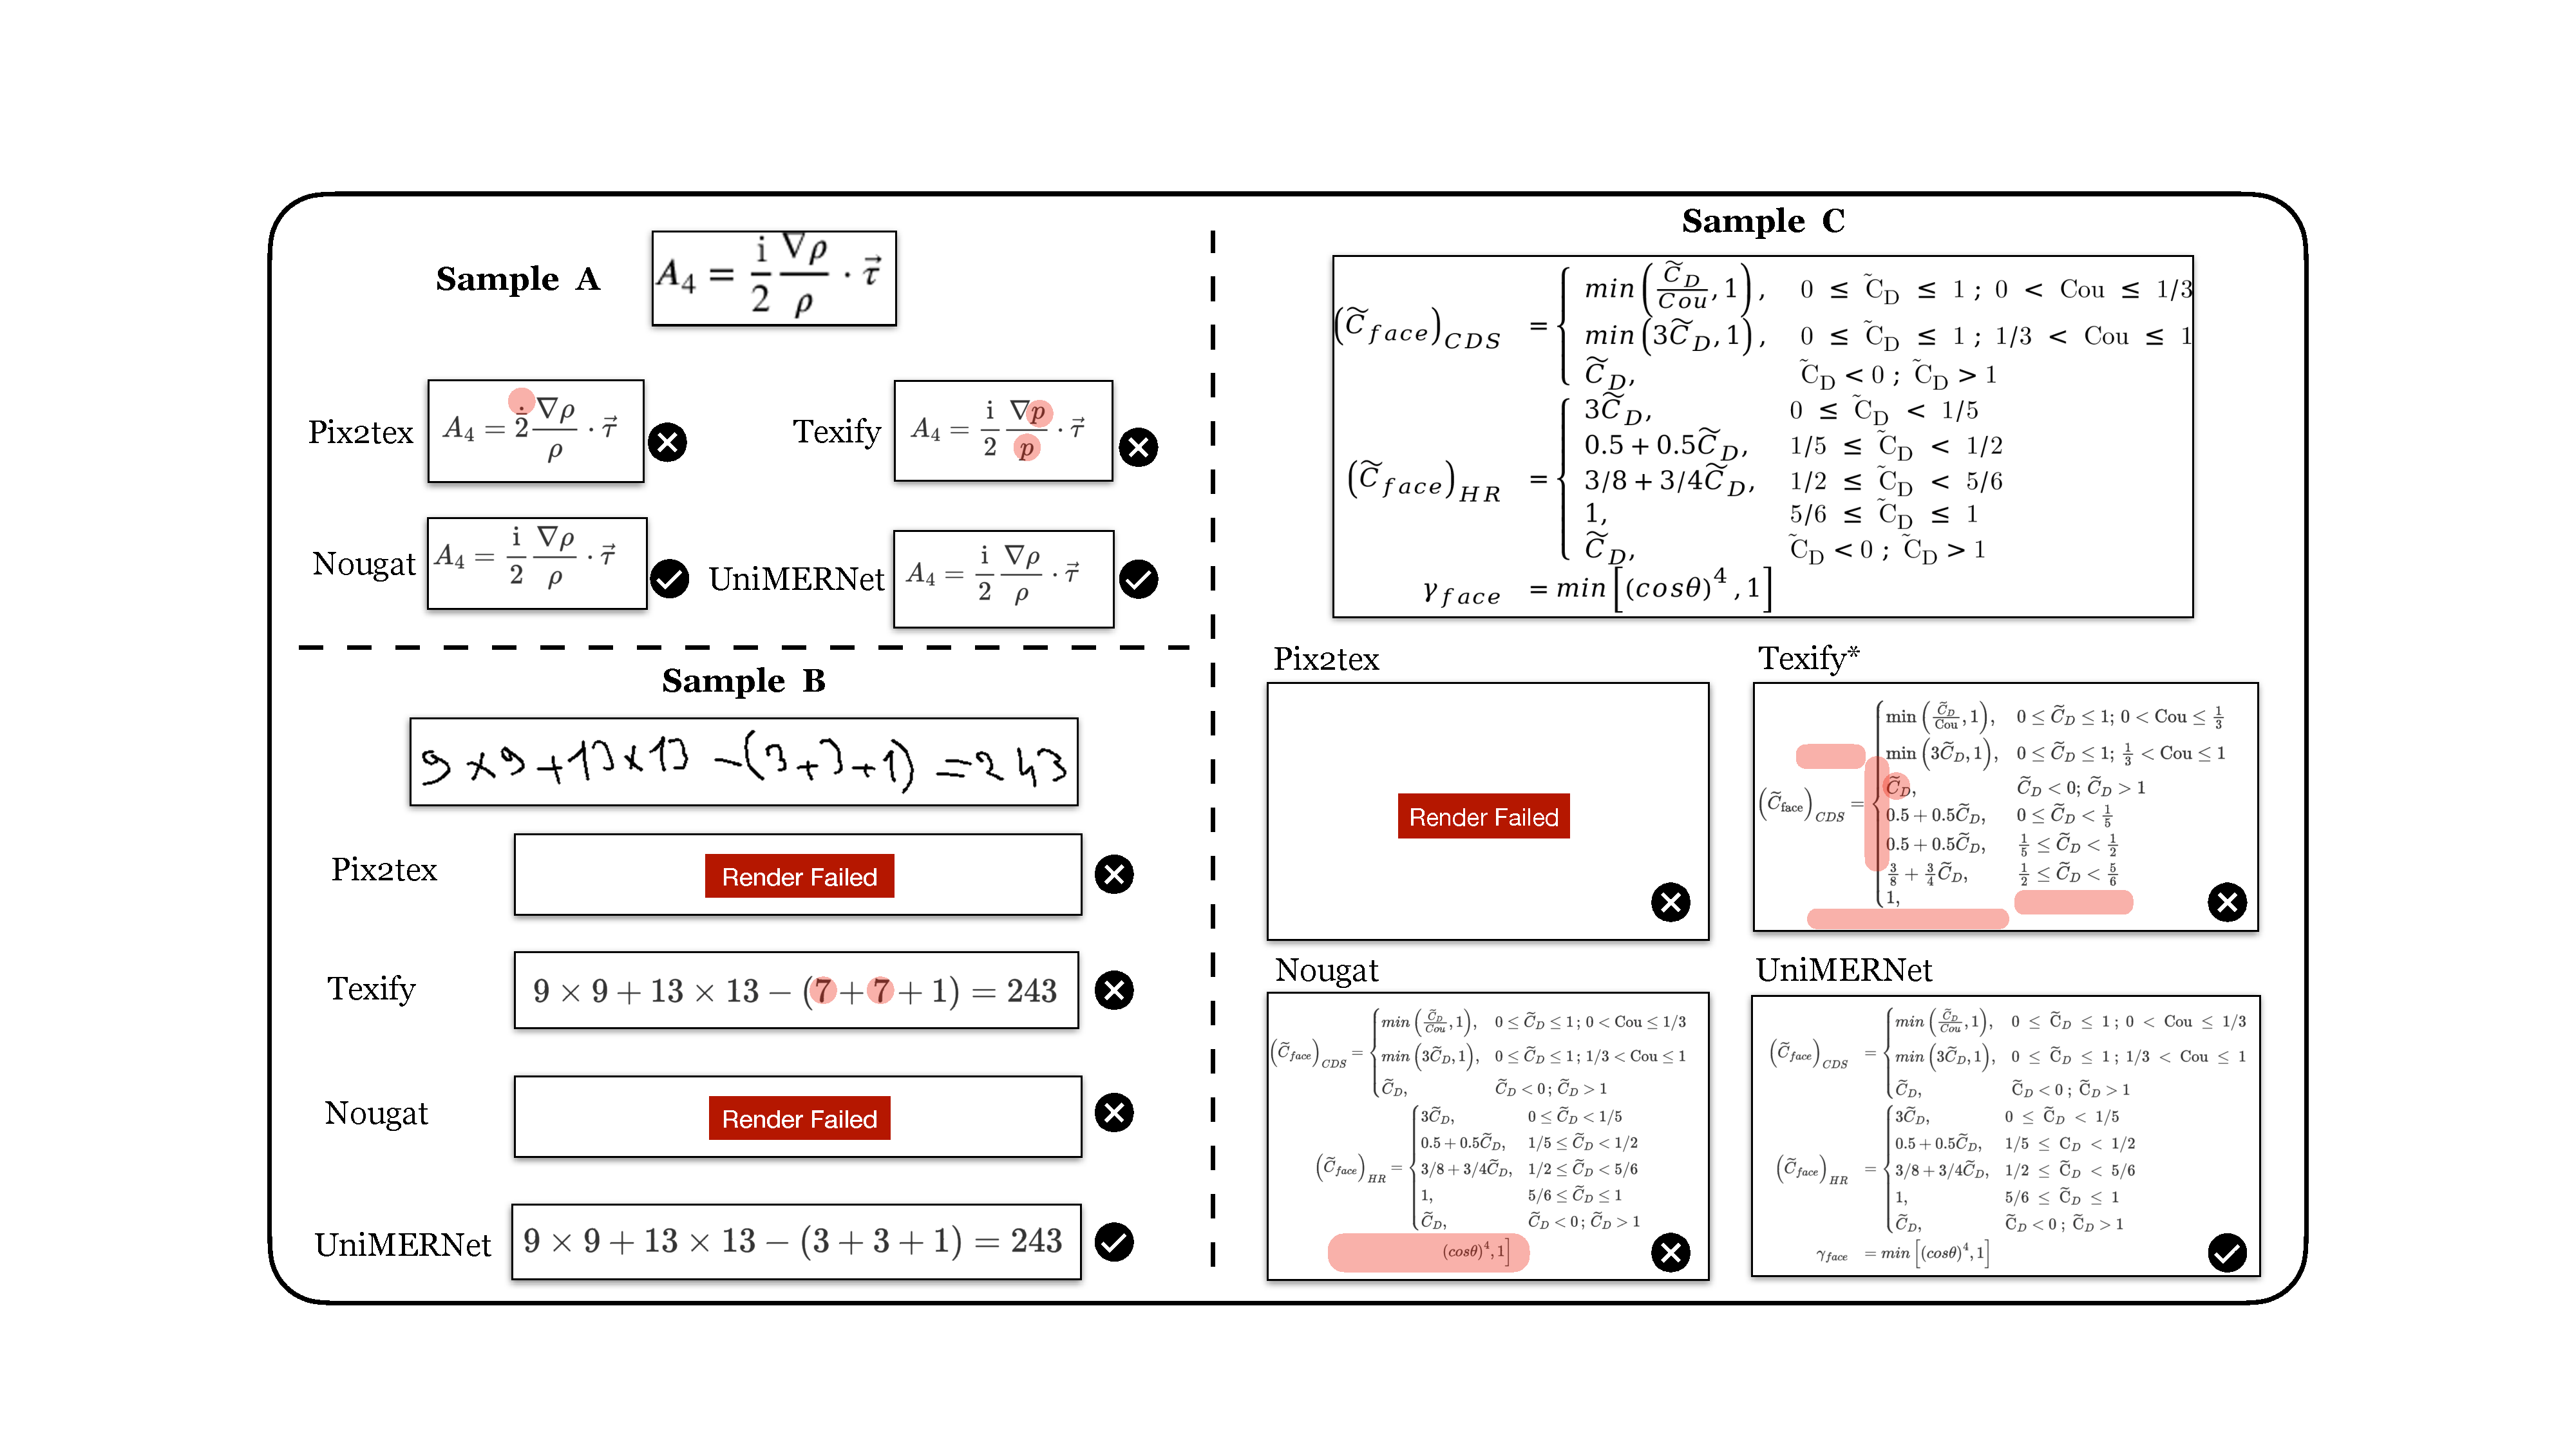
\includegraphics[width=0.95\linewidth]{figures/fig5_visualization.pdf}
    \caption{Comparative Visualization of Recognition Results Using Different Methods.}
  \label{fig:fig5_result}
  \vspace{-5pt}
\end{figure}


\vspace{-5pt}
\subsubsection{Comparison with Handwritten Expression Recognition Methods}

To fairly evaluate our model's ability to recognize handwritten formulas, we compared it with some of the most mainstream handwritten recognition models. As shown in ~\cref{tab:tab5}, although UniMERNet was not specifically optimized for handwritten formulas, it surpasses the SOTA handwritten recognition model across all CROHME test sets. On the CROHME 2014, CROHME 2016, CHOME 2019, and HME 100K test sets, UniMERNet achieves a completely accurate formula recognition rate (without any modifications) of 67.4\%, 68.4\%, and 65.4\%, outperforming the SOTA results on each dataset by 1.5\%, 5.3\%, and 1.1\% respectively. Furthermore, on the HME100K dataset, our model achieves comparable high-quality results to the specifically designed SOTA model.

\vspace{-5pt}
\subsubsection{Qualitative Comparisons}
As shown in \cref{fig:fig5_result},  we selected three representative samples from the UniMER-Test set to thoroughly compare the performance between Pix2tex~\cite{pix2tex2022}, Texify~\cite{texify2023}, Nougat~\cite{blecher2023nougat}, and UniMERNet. It's important to highlight that Nougat, being primarily designed for full-page recognition, tends to underperform with isolated formulas; thus, we prepared the test images by integrating random text with the formulas to adapt to Nougat's inference capabilities. Notably, while the other models exhibit certain shortcomings in handling these test samples, our model consistently delivers robust and accurate recognition results.


\section{Conclusion}
This research presents the UniMER-1M dataset and UniMER-Test, substantial contributions to the Mathematical Expression Recognition (MER) field, offering unprecedented scale and diversity. Our novel UniMERNet, validated through rigorous experimentation, sets a new benchmark in MER. The model's robustness and adaptability to varied lengths and noise levels underscore its practical value. Our resources are publicly available, aiming to catalyze further advancements in MER. Future work includes refining UniMERNet and exploring its fusion with LVLMs for holistic document understanding. This study represents a pivotal stride in MER, providing a robust foundation for future research.



%\clearpage\mbox{}Page \thepage\ of the manuscript. This is the last page.
\par\vfill\par
% Now we have reached the maximum length of an ECCV \ECCVyear{} submission (excluding references).
% References should start immediately after the main text, but can continue past p.\ 14 if needed.
\clearpage  % TODO REVIEW/FINAL: This \clearpage needs to be removed from both review and camera-ready versions.


% ---- Bibliography ----
%
% BibTeX users should specify bibliography style 'splncs04'.
% References will then be sorted and formatted in the correct style.
%
\bibliographystyle{splncs04}
\bibliography{main}
\end{document}
li